\section{Action Planning and Verification (Scott)}

The action planning process involves modeling the manipulator behavior and verifying a controller with respect to the model and any safety conditions specified by the user for a given action.
The trajectory planner is responsible for executing a rough motion of the manipulator to some approximate pose near the final desired location of the end effector (EFF).
In the case of the modular robot assembly, the trajectory planner moves the modular robot component to be attached to a location near the final attachment EFF pose.
The task planner provides the desired translation of the EFF in the global reference frame (necessary for making the connection) to the action planner, which then executes the motion once a controller has been verified.


\subsection{Continuous System Verification}
In order to avoid undesirable robot motions, the user specifies a set of unsafe states of the robot, $\varphi$, for a given action or motion of the manipulator.
For the case of modular robot assembly, the unsafe set is defined to be those poses of the end effector during an attachment motion that may result in a failed attachment or improper connection (magnet misalignment).
A given controller may be verified to cause the system remain within the safe set (no intersection with the unsafe set) by computing the set of all reachable states, $\textit{ReachSet}_{\mbox{\textit{H}}}$, from some initial condition ,$X_0 \subseteq X$.
However, determining the exact set of reachable states is difficult \cite{Henzinger:1995:WDH:225058.225162}, and an over approximation of the reachable set is instead computed.
The controller is verified if the over approximated set is contained within the set of states that satisfy the safety conditions, $\mbox{\textit{ReachSet}}_{\mbox{\textit{H}}} \subseteq \mbox{Sat}(\varphi)$.
The controller and motion are not verified if there is an intersection of the reachable states and the unsafe set, $\mbox{\textit{ReachSet}}_{\mbox{\textit{H}}} \cap \neg \mbox{Sat}(\varphi) \neq \emptyset$.
In the case where some intersection of the unsafe set and reachable set occurs, no conclusions may be drawn from the analysis as the reach set is an over approximation, and re-planning of the manipulator (by the trajectory planner) is required.

This process is similar to the framework in \cite{6016596}, in which the control architectures of an autonomous robotic surgery manipulator are verified for a puncturing task, whereby the EFF (puncturing instrument) is guaranteed to remain within some pose bounds.
In this work, the reachability tool Flow* \cite{Chen2013} is used to over approximate the system dynamics using Taylor Model flowpipes.
Flow* is capable of handling nonlinear systems, but as manipulators are highly nonlinear, the dynamics of the Baxter arms are linearized in an effort to increase computation speed. 


\subsection{Manipulator Modeling}
The dynamics of each of the Baxter arms can be represented as:
\begin{equation}
	\mathbf{M}(\underline{q})\ddot{\underline{q}} + \mathbf{C}(\underline{q},\underline{\dot{q}})\dot{\underline{q}} + \mathbf{G}(\underline{q}) = \underline{T}_{eff} + \underline{T}_{in}
\end{equation}
where $\mathbf{M}$ and $\mathbf{C}$ represent the inertial effects, $\mathbf{G}$ represents joint torques due to gravity, $\underline{T}_{EFF}$ represents the joint torques due to EFF load, and $\underline{T}_{in}$ represents the input joint torques.
In this case, linearizing the arm dynamics involves evaluating the nonlinear matrices $\mathbf{M}$, $\mathbf{C}$, and $\mathbf{G}$ for a given arm configuration.
As the action planner only executes arm motions for small EFF motions (and subsequently small changes in joint angle) it is assumed that these matrices remain constant for the duration of the arm motion executed by the action planner.
It should be noted that Coriolis effects, $\mathbf{C}$, are ignored due to the small motions of the arm.


\subsection{ROS Action Server and Code Diagram}
The action planner, comprising the reachability analysis, controller verification, and joint torque controller execution, are implemented as an action server in ROS.
The code block diagram is shown in figure Fig. \ref{fig:actionPlannerFlow}.
The action server, called by the task planner when a connection need to be performed, polls the current state of the arm holding the module to be attached, computes the linearized matrices of the manipulator equation, generates a Flow* file, performs the reachability computation for the given feedback controller, and then executes the motion if the controller/motion is verified.
The server creates an instance of Matlab when launched, which is then used for the kinematics computations and controller design.
The kinematics computations and linear model generation are done using the Matlab Robotics Toolbox \cite{Corke11a}.

Initially, the intent was to model the manipulator and controller(s) as a hybrid system, consisting of the continuous manipulator dynamics coupled with discrete controller states for aligning and approaching a connection.
However, the hybrid system model was discarded due to the complexity of developing a controller for the attachment motions.

\begin{figure}[h]
	\includegraphics[width = 8 cm]{action_server_2.png}
	\caption{Action Planner Module}
	\label{fig:actionPlannerFlow}
\end{figure}


\subsection{Difficulties with Baxter Joint Torque Control}
The initial controller used in the action planner server was a linear quadratic regulator (LQR) controller computed by Matlab.
The LQR controller provided feedback joint torques while a static input was added to counteract gravitational effects ($\mathbf{G}$ torques).
However, this controller, when implemented on the Baxter platform, resulted in erratic arm motions despite satisfactory performance in the Baxter simulator.
The Baxter platform provides a ``zero-gravity'' mode of operation whereby the robot continually provides torques to each joint sufficient to counteract gravitational effects.
The LQR controller, when implemented in ``zero-gravity'' mode (without the added gravitational torque compensation), resulted in arm ``drift,'' whereby the arm would slowly diverge from the initial condition.
Increasing the control effort did not improve the ability of the LQR controller to overcome the perceived arm ``drift.''
When the LQR controller was implemented with the ``zero-gravity'' mode disabled (during which the static gravitational torque inputs were included), the resulting arm motion was wildly erratic.
Operating with the ``zero-gravity'' mode disabled is not recommended.

The controller implemented in the final version of the action planner server (torque control) is a simple PD controller.
The Baxter robot has pre-defined joint spring and damping coefficients that can be called for PD joint torque control.
This controller (when used in ``zero-gravity'' mode) results in stable arm motion, both in simulation and on the physical robot.
However, the default spring and damping values result in significant arm oscillations when the robot is moving from one configuration to another.
As oscillations are undesirable when connecting modular components, the damping values are increased.
It should be noted that both the spring and damping coefficient values are passed in to the action planner server when called and, as such, may be altered at runtime by the task planner.

\subsection{Verified Motion Example}
The results of the execution of a simple motion command on the left arm by the action planner are shown in Figures \ref{fig:effX},\ref{fig:effY}, and \ref{fig:effZ}.
In this example, the input desired EFF motion is appx. 10 cm in the negative z direction (toward the ground) in the Baxter global reference frame, starting in the neutral arm position.
The values plotted are with respect to the starting $x/y/z$ EFF position.

\begin{figure}[h]
	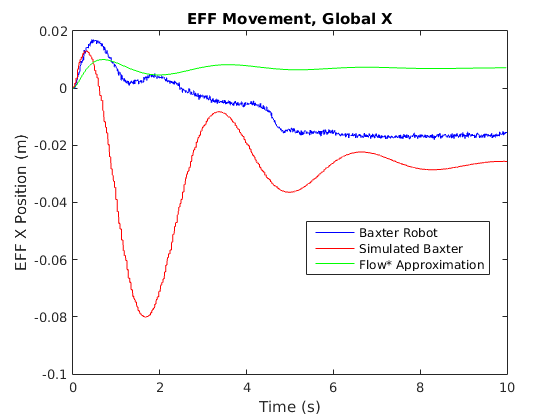
\includegraphics[width = 9 cm]{effx_example.png}
	\caption{Example Action Planner Execution, EFF $X$ motion}
	\label{fig:effX}
\end{figure}

\begin{figure}[h]
	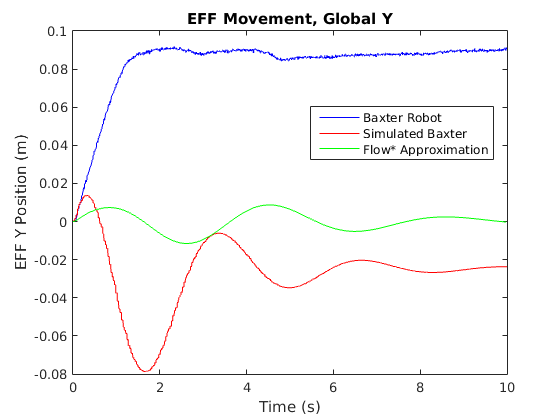
\includegraphics[width = 9 cm]{effy_example.png}
	\caption{Example Action Planner Execution, EFF $Y$ motion}
	\label{fig:effY}
\end{figure}

\begin{figure}[h]
	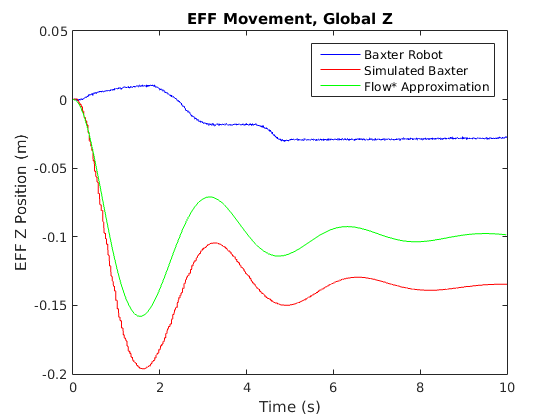
\includegraphics[width = 9 cm]{effz_example.png}
	\caption{Example Action Planner Execution, EFF $Z$ motion}
	\label{fig:effZ}
\end{figure}

The Flow* approximations, shown in green, show the computed reachable set for each EFF position variable $(x,y,z)$ as a function of time.
The range of the reachable set are small at each time step as the initial conditions for the computation are scalar values rather than a range.
Given a range of initial conditions (representing, for example, error in the measured joint angles) the computed reachable sets would show a greater range of values - the green lines wold appear more like funnels showing the over approximated upper and lower bounds for the variables.
The reachable sets shown here are computed with scalar initial conditions for clarity.

The reachable sets computed from the linear model predict small deviations ($<$ 2 cm) of the $x$ and $y$ EFF values during the motion and show the $z$ value converging to the desired value of -0.1, albeit with some oscillation.
Despite the near 5 cm overshoot in the $z$ direction predicted by the linear model, the small predicted $x$ and $y$ deviations may be sufficient for a successfully attaching a module.
However, the EFF motions recorded in the Baxter simulator and physical robot clearly do not agree with the predicted motions.
The data from the simulated Baxter robot shows significantly increased oscillations and the data from the physical robot shows stiff, heavily damped motions.
The motions of the physical robot during the execution of the action planner were observed to be stiff, jerky, and unrepeatable, likely due to significant, asymmetric friction in the arm joints.
Increasing the damping control term increased the stiff, jerky arm motions and decreasing the damping term resulted in continual oscillations - the damping parameter was ``tuned'' but ultimately the arm behavior was to erratic to be effective.
As such, the output of the reachable set computation is not valid in this case for determining the safety of a given controller.


\subsection{First Order Joint Control for Demonstration}
A first order (joint speed) controller was implemented in an effort to avoid the erratic behavior of the LQR and PD joint torque controllers.
Using the global reference frame Jacobian computed in the Matlab Robotics Toolbox, the required joint velocities are computed for a desired end effector translation.
This controller was used for the demonstration examples.

\subsection{Action Planner - Successes and Failures}
The implementation of the action planner as a ROS action server, integration of Matlab and the Robotics Toolbox, and Flow* model generation and computation were all successful during this project.
However, the torque controller developed for this work was ultimately unsuccessful due to the erratic and unpredictable nature of the arm motions during joint torque control.
Future work on developing an effective joint torque controller for the Baxter robot should focus on characterizing each arm joint with respect to friction and damping.
This characterization may allow for properly determining the PD stiffness and damping terms for each joint for a given motion.

In addition, future work should focus on the validity of the linearized manipulator model.
Bounding the error of the linearizion will allow the reachability computation to formally verify the controller/motion.





\begin{comment}
The action planning stage of the assembly process is broken down into two parts: modeling the manipulator behavior as a hybrid system and verifying safety conditions of the end effector motions (making sure that undesirable motions do not occur).

\subsection{Hybrid system modeling}
The trajectory planner discussed in the previous section is responsible for moving each arm (trajectory execution) to within some bound of the final desired end effector position (determined by the task planner) for either (i) grasping or (ii) component alignment. 
The trajectory planner provides to the action planner the final positions of the end effectors with respect to the appropriate blocks for (i) grasping, or (ii) alignment at attachment.
In either case, it is beneficial to avoid damaging a robot module or failing to complete a grasp or attachment due to position and alignment errors.
For the proposed scenario of assembling modular robotic components, we implement a system similar to a framework \cite{6016596} developed to address the verification of control architectures for autonomous robotic surgery manipulation tasks with respect to various safety conditions, denoted as $\varphi$, such as avoiding end effector misalignment or excessive force application.

In the previously mentioned framework, the system is modeled as a hybrid automaton \cite{Alur1993}, composed of discrete states (tasks/behaviors) and continuous dynamics associated with each state or behavior.
In our case of modular robot assembly, each state consists of \textit{fast approach}, which is handled by the trajectory planner, and \textit{slow approach}, \textit{alignment}, \textit{grasping}, and \textit{connecting}, handled by the action planner. 
Each state also contains a controller, a set of invariants (conditions required to be true while the automaton is in that state), and a set of guards (conditions that must be true in order for a state transition to take place).

\subsection{Verification of Behaviors}
In order to verify that the safety conditions $\varphi$ are satisfied for the discrete state controllers, the reachable set of the system $\textit{ReachSet}_{\mbox{\textit{H}}}$, which is the set of all reachable states from some initial condition, $X_0$, can be compared to the set of states for which the safety properties are not satisfied, $\neg \mbox{Sat}(\varphi)$.
However, computing the exact set of reachable states is difficult \cite{Henzinger:1995:WDH:225058.225162} and approximations may be used instead.
In this case, a reachability tool (e.g. \textit{SpaceEx}~\cite{rehseGDCRLRGDM11}), which computes approximate reachable sets given the system dynamics and controllers, can be used to over-approximate the reachable set of the hybrid system $\textit{ReachSet}_{\mbox{\textit{H}}}$ such that $\mbox{\textit{ReachSet}}_{\mbox{\textit{H}}} \supseteq \mbox{Sat}(\varphi)$, where $\mbox{Sat}(\varphi)$ is the set of states that satisfies $\varphi$.
If $\mbox{\textit{ReachSet}}_{\mbox{\textit{H}}}$ does not intersect with the set of states for which the safety conditions $\varphi$ is not satisfied, $\mbox{\textit{ReachSet}}_{\mbox{\textit{H}}} \cap \neg \mbox{Sat}(\varphi) = \emptyset$, the safety of the system is verified.

In the case that $\mbox{\textit{ReachSet}}_{\mbox{\textit{H}}} \cap \neg \mbox{Sat}(\varphi) \neq \emptyset$, the inconclusive nature of the system is communicated to the trajectory planner and the system will either (i) re-plan the arm motions or (ii) adjust the boundaries specified in the safety conditions, $\varphi$ and recompute the system reachability.

\end{comment}

